% This is samplepaper.tex, a sample chapter demonstrating the
% LLNCS macro package for Springer Computer Science proceedings;
% Version 2.20 of 2017/10/04
%
\documentclass[runningheads]{llncs}
%
\usepackage{graphicx}
\usepackage{color}
\usepackage{hyperref}

\usepackage{amsmath}

% Used for displaying a sample figure. If possible, figure files should
% be included in EPS format.
%
% If you use the hyperref package, please uncomment the following line
% to display URLs in blue roman font according to Springer's eBook style:
% \renewcommand\UrlFont{\color{blue}\rmfamily}

\begin{document}
%
\title{ML-based approach for accelerating global search algorithm for solving multicriteria problems\thanks{Supported by organization x.}}
%
%\titlerunning{Abbreviated paper title}
% If the paper title is too long for the running head, you can set
% an abbreviated paper title here
%
\author{Konstantin Barkalov\orcidID{0000-0001-5273-2471} \and
Vladimir Grishagin\orcidID{0000-0002-2884-3670} \and
Evgeny Kozinov\orcidID{0000-0001-6776-0096}}
%
\authorrunning{K. Barkalov, V. Grishagin and E. Kozinov}
% First names are abbreviated in the running head.
% If there are more than two authors, 'et al.' is used.
%
\institute{Lobachevsky State University of Nizhni Novgorod, Nizhni Novgorod, Russia \email{\{konstantin.barkalov,evgeny.kozinov\}@itmm.unn.ru}, \email{vagris@unn.ru}}
%
\maketitle              % typeset the header of the contribution
%
\begin{abstract}
The paper considers a new approach to solving multicriterial optimization problems on the base of criteria scalarization, dimensionality reduction via Peano curves and efficient global search algorithm. The novelty of the approach consists in application of machine learning methods combined with utilizing a posteriori information for acceleration of the search. Effectiveness of the proposed approach has been demonstrated by means of solving a set of multiextremal multicriterial optimization problems.

\keywords{Multicriterial Problems \and Global Optimization \and Machine Learning \and Logistic Regression.}
\end{abstract}
%
%
%
\section{Introduction}
\textcolor[rgb]{1,0,0}{Machine learning (ML) methods are powerful tools that are applied in many areas of research.}
In particular, the ML methods are successfully used for solving complicated problems of computational mathematics. One of such problem classes to which ML can be applied is the class of multicriterial optimization (MCO) models. 
In this case, ML is used, as a rule, in combination with metaheuristic algorithms \cite{Subraveti2019} that in the case of multiextremal criteria lose in efficiency to deterministic methods \cite{Kvasov2018,Sergeyev2018}.

Among the most qualitative deterministic methods for solving \textcolor[rgb]{1,0,0}{these problems} the information-statistical global search algorithm \cite{Sergeyev2013,Strongin2000} can be considered. This method proposed initially for solving scalar problems was successfully extended to MCO models \cite{GergelKozinovAPI2016,Gergel2018}.

The paper reflects results of a new research direction connected with utilizing ML methods for acceleration of the global search algorithm in the case of its application to MCO problems. The proposed approach is based on building a number of separation planes in the criteria space to segregate the Pareto set and accelerate the process of its construction. The efficiency of the approach is estimated experimentally compared to several other MCO methods.


\section{Problem statement}

The MCO problem to be considered is formulated as follows:
\begin{equation}
f(y)=(f_1 (y),f_2 (y),\dots ,f_s (y)) \to \min, \; y\in D,
\label{eq:1}
\end{equation}
\begin{equation}
D=\left\{ y \in R^N: a_i \leq y_i \leq b_i, \; 1 \leq i \leq N, \; a,b \in R \right\}.
\label{eq:2}
\end{equation}
where $f_i (y)$, $1 \leq i \leq s$, are  criteria, $y=(y_1,y_2, \dots,y_N)$ is a vector of independent variables, $N$ is the dimension of the problem. The criteria $f_i (y)$, $1 \leq i \leq s$, are supposed to be multiextremal, to be given as a ``black-box'' functions and to satisfy the Lipschitz condition
\begin{equation}
|f_i (y')-f_i (y'')| \leq L_i \|y'-y''\|, \; y',y'' \in D, \; 1 \leq i \leq s,
\label{eq:3}
\end{equation}
where $L_i>0$, $1 \leq i \leq s$, are a priori unknown Lipschitz constants.

Any effective (Pareto-optimal) variant  in which it is impossible to reduce the values of all criteria $f_i (y)$, $1 \leq i \leq s$, at once by choosing another option   can be considered as a partial solution to the MCO problem. In practice, various scalarization techniques are often used to find effective solutions \cite{Ehrgott2005,Pardalos2017,Marler2004,GergelKozinov2020}. The present study uses the minimax convolution of partial criteria that possesses good theoretical properties
\begin{equation}
\min{f(y)} \to \min_{y\in D}{\max_{1 \leq i \leq s}{(f_i (y) \lambda_i )}} ,
\label{eq:4}
\end{equation}
where $\lambda_i \geq 0$, $1 \leq i \leq s$, $\sum_{i=1}^s{\lambda_i}=1$, are numerical indicators of the significance of each criterion. 

In general case, the entire set of Pareto-optimal variants is taken as a complete solution to the MCO problem. For the numerical building of an approximation of the Pareto set a number of scalar optimization problems (\ref{eq:4}) are solved with different coefficients $\lambda_i \geq 0$, $1 \leq i \leq s$, uniformly distributed
%in the space of ones.
\textcolor[rgb]{1,0,0}{in $[0,1]$.}

\section{General computational scheme}

In the framework of the proposed approach the information-statistical theory of global search is used for solving the scalar optimization problems (\ref{eq:4}). For problems with several variables ($N>1$) the dimensionality reduction on the base of Peano-type mappings \cite{Sergeyev2013,Strongin2000}. While solving a problem (\ref{eq:4}) the algorithm generates a sequence of trials where the term ``trial'' means evaluation of criteria at a point of the feasible domain D and computation of the convolution (\ref{eq:4}) at this point. 

Coordinates of a new trial are chosen according to the following rules: 

\begin{enumerate}
  \item Obtain univariate images of all points of preceding trials mapped onto one-dimensional interval [0,1] by means of Peano curves.
  \item Partition the segment [0,1] into subintervals according to the images of trials performed.
  \item For each subinterval compute a numerical value called \textit{characteristic} of this subinterval.
  \item Select the subinterval with the highest characteristic.
  \item Place the point of new trial within the subinterval with the highest characteristic. 
  \item Map the new trial point to the point $y \in D$ using Peano evolvent and compute the value of the function (\ref{eq:4}) at this point. 
\end{enumerate}

The algorithm completes execution when the required accuracy is achieved. After stopping the global search algorithm, an estimate of the Pareto set is built on the base of the accumulated information obtained in the course of optimization. If the quality of the Pareto set estimate is not sufficient, then new preferences (new coefficients $\lambda$) are set and the search process continues.

\section{Approaches to improving search efficiency}

Two techniques are used to improve the search efficiency of the Pareto area assessment. 

The first one is to jointly solve a series of global search problems from (\ref{eq:4}). The essence of the technique consists in the accumulation of search information during the optimization process and in reusing afterwards this information while solving a problem (\ref{eq:4}) with new weight coefficients $\lambda$. A detailed description of the technique can be found in \cite{GergelKozinovAPI2016,Gergel2018}.

The second improvement is connected with a new method for calculating the characteristics of subintervals formed during univariate optimization on the internal [0,1].

Let $R(i)$ be the characteristic of the $i$-th subinterval. This characteristic is supposed to consist of two parts:

\begin{equation}
R(i)=R_{ags} (i)+ \alpha R_{PS} (i).
\label{eq:5}
\end{equation}

The term $R_{ags}(i)$ allows you to select a subinterval oriented at finding the global minimum of the current optimization task (\ref{eq:4}), while $R_{PS}(i)$ influences the selection of a subinterval to improve the evaluation of the Pareto area. The coefficient $\alpha$ from (\ref{eq:5}) allows adjusting the contribution of each of parts.

$R_{ags}(i)$ is calculated in accordance with the expression from the global search algorithm \cite{GergelKozinovAPI2016,Gergel2018,Sergeyev2013,Strongin2000}.

Calculation of $R_{PS}(i)$ is based on machine learning methods. When solving the first global search problem (\ref{eq:4}), the value of $R_{PS}(i)$ is assumed to be zero. To solve each subsequent scalar problem (\ref{eq:4}), $R_{PS}(i)$ is calculated as follows.

In the course of Pareto set assessment all trial points are partitioned into two classes. This bipartition is based on belonging to the Pareto set. For these classes, a separation hyperplane is constructed in the domain of criteria values using the logistic regression \cite{Yu2011}. Examples of separated planes are shown in Fig. \ref{fig:1}. During the choice of a new trial point, the distances of all obtained criteria values from the separated plane are calculated and the value of $R_{PS}(i)$ is built depending on these distances. 

\begin{figure}[ht]
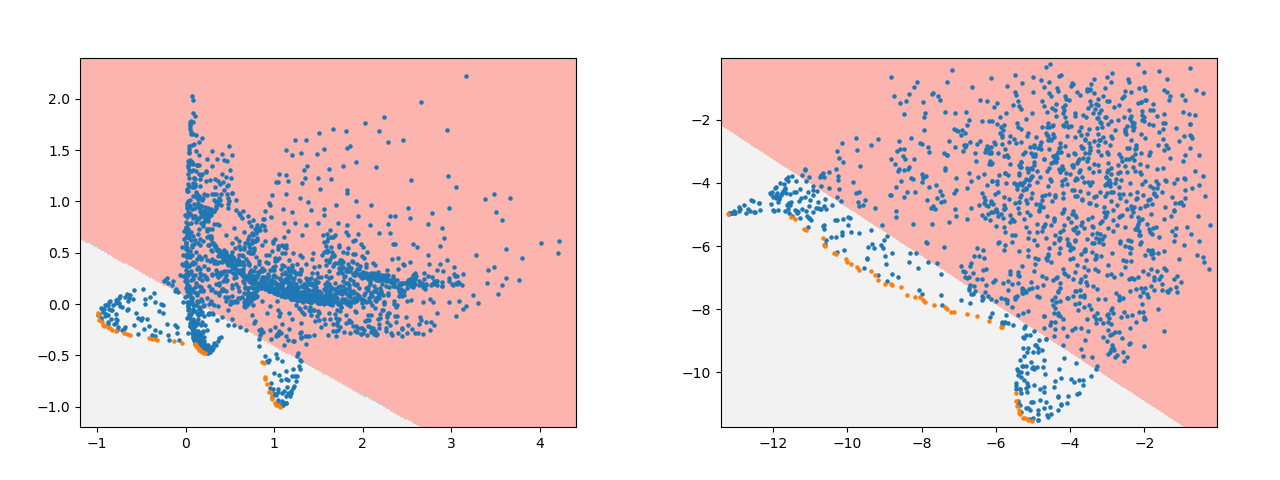
\includegraphics[width=0.8\textwidth]{fig1.png}
\caption{Separated hyperplanes in the criteria space} \label{fig:1}
\end{figure}

Hereinafter the algorithm taking into account distances to separated hyperplane and accumulated information will be called ML\_MGSA.

\section{Results of computational experiments}

Computational testing was carried out on the supercomputer ``Lobachevsky'' of Nizhny Novgorod State University in the environment of the Globalizer software system \cite{globalizerSystem}. 

The first series of experiments was performed to compare the algorithm ML\_MGSA with a number of widely known multiobjective optimization algorithms using a test two-criterion problem \cite{Evtushenko2014}

\begin{equation}
f_1 (y) = (y_1-1) y_2^2+1, f_2 (y) = y_2, 0\leq y_1, y_2 \leq 1.
\label{eq:6}
\end{equation}

In these experiments, a numerical approximation of the Pareto set was built. The quality of approximation is estimated by such indicators as the hypervolume index (HV) and distribution uniformity index (DU) \cite{Evtushenko2014,Zilinskas2015}. In the framework of the experiment 5 algorithms of multicriterial optimization were compared: the Monte-Carlo (MC) method, the genetic algorithm SEMO \cite{PISA2003}, the Non-uniform coverage (NUC) method \cite{Evtushenko2014}, the bi-objective Lipschitz optimization (BLO) method \cite{Zilinskas2015} and algorithm ML\_MGSA, proposed in this article. 
  
ML\_MGSA solved 25 problems (\ref{eq:4}) with different convolution coefficients $\lambda$, uniformly distributed in the field of their variation. The results of the conducted experiments are shown in Table \ref{tab:1} where ML\_MGSA with $\alpha=0$ corresponds to the version without machine learning.

\begin{table}[]
\caption{Efficiency of the multicriterial algorithms compared}
\label{tab:1}
\begin{tabular}{ccccccc}
\hline
Algorithm                      & MC    & SEMO  & NUC   & BLO   & \begin{tabular}[c]{@{}c@{}}ML\_MGSA \\ ($\alpha= 0$)\end{tabular} & \begin{tabular}[c]{@{}c@{}}ML\_MGSA \\ ($\alpha= 1.5$)\end{tabular} \\ \hline
Number of trials               & 500   & 500   & 515   & 498   & 302             & 269               \\
Number of Pareto points found  & 67    & 104   & 29    & 68    & 92              & 79                \\
HV index (the more the better) & 0.300 & 0.312 & 0.306 & 0.308 & 0.312           & 0.312             \\
DU index (the less the better) & 1.277 & 1.116 & 0.210 & 0.175 & 0.101           & 0.103             \\ \hline
\end{tabular}
\end{table}

As it follows from the results presented in Table \ref{tab:1}, ML\_MGSA demonstrates the better quality compared to other methods.

In the second group of experiments 100 bi-criteria MCO problems have been solved. As the criteria the multiextremal functions

\begin{equation}
\begin{matrix}
f(y) = - (AB + CD)^{1/2} \\
AB = \Big(\sum_{i=1}^7 \sum_{j=1}^7 [A_{ij} a_{ij}(y_1, y_2) + B_{ij} b_{ij}(y_1, y_2)]\Big)^2 \\
CD = \Big(\sum_{i=1}^7 \sum_{j=1}^7 [C_{ij} a_{ij}(y_1, y_2) - D_{ij} b_{ij}(y_1, y_2)]\Big)^2 \\ 
a_{ij}(y_1, y_2) = \sin(\pi i y_1) \sin(\pi j y_2), b_{ij}(y_1, y_2) = \cos(\pi i y_1) \cos(\pi j y_2),
\end{matrix}
\end{equation}
$0 \leq y_1,y_2 \leq 1$, have been taken where parameters $-1 \leq A_{ij},B_{ij},C_{ij},D_{ij} \leq 1$ are the independent random numbers distributed uniformly \cite{Grishagin2015_2,Gergel2019_2}.

In order to estimate efficiency of machine learning procedure in ML\_MGSA, this method tested in 2 variants: with ($\alpha>0$) and without ($\alpha=0$) machine learning. Each multicriterial problem was reduced to 50 scalar problems (\ref{eq:4}) with different weight coefficients $\lambda$ distributed uniformly. Other algorithm's parameters were the same. The averaged results can be found in Table \ref{tab:2}.

\begin{table}[]
\caption{Efficiency of the multicriterial algorithms compared}
\label{tab:2}
\begin{tabular}{ccc}
\hline
                                  & ML\_MGSA ($\alpha=0.0$) & ML\_MGSA ($\alpha=0.01$) \\ \hline
Average number of iterations      & 1902.4           & 658.6             \\
Average value of  DU index        & 1.32             & 1.55              \\
Average value of HV index         & 92.1             & 91.9              \\
Reducing the number of iterations & 1                & 2.9     \\  \hline        
\end{tabular}
\end{table}

As shown in the table, embedding the machine learning into the global search algorithm results in a significant reduction of the number of trials (almost 3 times) with maintaining close values of indicators HV and DU.

%1 \cite{Miettinen1999}
%2 \cite{Ehrgott2005}
%3 \cite{Pardalos2017}
%4 \cite{Strongin2000}
%5 \cite{Sergeyev2013}
%6 \cite{GergelKozinovAPI2016}
%7 \cite{Gergel2018}
%8 \cite{Marler2004}
%9 \cite{GergelKozinov2020}
%10 \cite{Yu2011}
%11 \cite{globalizerSystem}
%12 \cite{Evtushenko2014}
%13 \cite{Zilinskas2015}
%14 \cite{PISA2003}


%
% ---- Bibliography ----
%
% BibTeX users should specify bibliography style 'splncs04'.
% References will then be sorted and formatted in the correct style.
%
% \bibliographystyle{splncs04}
% \bibliography{mybibliography}
%
\bibliographystyle{splncs04}
\bibliography{bibliography}

\end{document}
